\documentclass{article}
\usepackage{jfrExamplee}
\usepackage{graphicx}
\usepackage{apalike}
\usepackage{setspace}

%% Uncomment line below for double spacing
%\doublespacing

%this template built off template for NIPS 2004

\title{A Single Wheel Test Rig for Ocean World Rovers}

\author{
Athul Pradeepkumar Girija\thanks{ Use footnote for providing further information
about author (webpage, alternative address). Acknowledgments to
funding agencies should go in the \textbf{Acknowledgments} section
at the end of the paper.} \\
School of Aeronautics and Astronautics\\
Purdue University\\
West Lafayette, IN 47907 \\
\texttt{apradee@purdue.edu} \\
\And
Ye Lu \\
School of Aeronautics and Astronautics \\
Purdue University \\
West Lafayette, IN 47907 \\
\texttt{yelu@purdue.edu} \\
\And
Archit Arora \\
School of Aeronautics and Astronautics \\
Purdue University \\
West Lafayette, IN 47907 \\
\texttt{arora31@purdue.edu} \\
\And
Rachana Agrawal \\
School of Aeronautics and Astronautics \\
Purdue University \\
West Lafayette, IN 47907 \\
\texttt{agrawa77@purdue.edu} \\
\And
Maxim de Jong \\
Thin Red Line Aerospace \\
Chilliwack, British Columbia\\ V2R 5M3, Canada\\
\texttt{maxim@thin-red-line.com} \\
\And
Matt Kent \\
Materials Science and Engineering\\
Smithers \\
Ravenna, Ohio 44266\\
\texttt{mkent@smithers.com} \\
\And
Sarag J. Saikia \\
School of Aeronautics and Astronautics \\
Purdue University \\
West Lafayette, IN 47907 \\
\texttt{ssaikia@purdue.edu} \\
\And
James M. Longuski \\
School of Aeronautics and Astronautics \\
Purdue University \\
West Lafayette, IN 47907 \\
\texttt{longuski@purdue.edu} \\
}

% The \author macro works with any number of authors. There are two commands
% used to separate the names and addresses of multiple authors: \And and \AND.
%
% Using \And between authors leaves it to \LaTeX{} to determine where to break
% the lines. Using \AND forces a linebreak at that point. So, if \LaTeX{}
% puts 3 of 4 authors names on the first line, and the last on the second
% line, try using \AND instead of \And before the third author name.

\begin{document}

\maketitle

\begin{abstract}
Sed ut perspiciatis unde omnis iste natus error sit voluptatem accusantium doloremque laudantium, totam rem aperiam, eaque ipsa quae ab illo inventore veritatis et quasi architecto beatae vitae dicta sunt explicabo. Nemo enim ipsam voluptatem quia voluptas sit aspernatur aut odit aut fugit, sed quia consequuntur magni dolores eos qui ratione voluptatem sequi nesciunt. Neque porro quisquam est, qui dolorem ipsum quia dolor sit amet, consectetur, adipisci velit, sed quia non numquam eius modi tempora incidunt ut labore et dolore magnam aliquam quaerat voluptatem. Ut enim ad minima veniam, quis nostrum exercitationem ullam corporis suscipit laboriosam, nisi ut aliquid ex ea commodi consequatur? Quis autem vel eum iure reprehenderit qui in ea voluptate velit esse quam nihil molestiae consequatur, vel illum qui dolorem eum fugiat quo voluptas nulla pariatur? At vero eos et accusamus et iusto odio dignissimos ducimus qui blanditiis praesentium voluptatum deleniti atque corrupti quos dolores et quas molestias excepturi sint occaecati cupiditate non provident, similique sunt in culpa qui officia deserunt mollitia animi, id est laborum et dolorum fuga. Et harum quidem rerum facilis est et expedita distinctio. Nam libero tempore, cum soluta nobis est eligendi optio cumque nihil impedit quo minus id quod maximes.
\end{abstract}

\section{Introduction}
Mobility systems have proven to be of immense value in in-situ planetary exploration over the last five decades since Lunokhod-1, the first successful rover to operate on the lunar surface in 1970 \cite{sanguino201750,kassel1971lunokhod}. As opposed to orbital platforms which can only perform remote-sensing investigations and static landers which provide in-situ data but only for a single site, mobility systems enable in-situ measurements across a range of scientifically interesting sites. A wide range of mobility systems which include rovers, articulated robots, hoppers, helicopters, multicopters, balloons, airplanes, floating platforms, ice drills, and submersibles have been proposed for planetary exploration across the Solar System \cite{iagnemma2004mobile,preumont1997conceptual,fiorini1999hopping,balaram2018mars,hassanalian2018evolution,yajima2009scientific,landis2005venus,mitri2014exploration,weiss2008study,lorenz2018exploring}. 

At the time of writing, NASA's Curiosity rover is operational on the Martian surface since 2012 and the Perseverance rover is scheduled to arrive at Mars in 2021 \cite{welch2013systems,williford2018nasa}. The European Space Agency's Rosalind Franklin rover is scheduled to arrive at Mars in 2022 \cite{vago2017habitability}. The Chinese National Space Agency's Yutu 2 rover is operational on the lunar far side and has become the longest operational lunar rover, breaking Lunokhod-1's previous record of 10.5 months \cite{ling2019close}.

The continued interest and commitment in surface mobility systems despite their inherently higher costs compared to orbiter and lander missions underscore their importance in future planetary exploration. However, the poorly known surface properties and features (loose sand, large boulders, sharp rocks etc.) present significant engineering challenges to surface mobility systems. Perhaps the most notable example is NASA's Spirit rover became trapped in soft sand and could not gain traction to free itself, eventually leading to a loss of mission \cite{lorenz2014moving}. Prior to the embedding event, the Spirit rover had experienced significant slippage when crossing fine-grained surfaces \cite{li2008characterization}. The twin rover Opportunity has also been subject to such near-embedding events as it traversed deformable sand terrain \cite{zhou2014simulations,arvidson2011opportunity}. Similar slippage and sinkage problems were encountered by the Curiosity rover when crossing ripple fields \cite{arvidson2014roving}; in addition to significant wheel damage from traversing over sharp rock outcrops \cite{arvidson2017relating}. These experiences make it clear that a thorough understanding of the wheel-soil/terrain interaction is of critical importance for planning future missions which include surface mobility systems. The Mars rovers used a combination of numerical modeling, single-wheel test rig experiments, and full vehicle field tests in analog sites such as the Mojave Desert to characterize the wheel-terrain interaction and predict vehicle performance. Based on the data, the mission operations team selects the best possible path so as to minimize the risk of undesirable events such as embedding in a sand trap.

While the majority of the existing literature in the field of planetary rovers focus on the Moon and Mars, the Ocean Worlds such as Europa and Enceladus in the outer Solar System are potential targets for in-situ exploration in the near future \cite{sherwood2018program}. These worlds are known to harbor massive liquid water oceans underneath their icy crust, and are prime candidates in the search of life beyond Earth \cite{nimmo2016ocean}. Multiple studies have investigated the scientific potential and technical challenges of lander and mobile platforms on Europa and Enceladus \cite{pappalardo2013science,patthoff2018science,hand2017report,hobley2013rough,nayar2017surface}. Ocean Worlds such as Europa present a significantly more challenging environment compared to Mars due to the extremely cold temperature, high radiation dosage, and the poorly constrained material properties under these conditions. Preliminary studies using photopolarimetric observations suggest that granular ice under cryogenic and vacuum conditions may be extremely fine grained material and is a potential hazard to landed spacecraft \cite{nelson2018laboratory}. Other potential hazards include penitent-like formations which create sharp ice outcrops \cite{hobley2018formation}; or massive boulder fields as seen by Cassini during close flybys of Enceladus \cite{porco2006cassini}. Researchers at Purdue University have developed a unique single wheel test rig to characterize wheel terrain interactions for future Ocean World mobility systems. The test-rig accommodates tires as large as 2 meters in diameter, and features a test-bed which can simulate varied surface features such as fine grained ice, smooth hard ice, sharp rock formations and boulder outcrops of a range of size distributions. This paper describes the design, capabilities, and initial results from the Purdue single wheel test rig for Ocean World rovers. 









\section{A Brief Survey of Existing Planetary Rover Test Rigs}
Test text to check commit changes.


\section{Design and Fabrication of the Single-Wheel Test Rig}





\section{Tire Prototype Fabrication}

\section{Experimental Setup and Procedure}
\begin{figure}[hbt!]
\centering
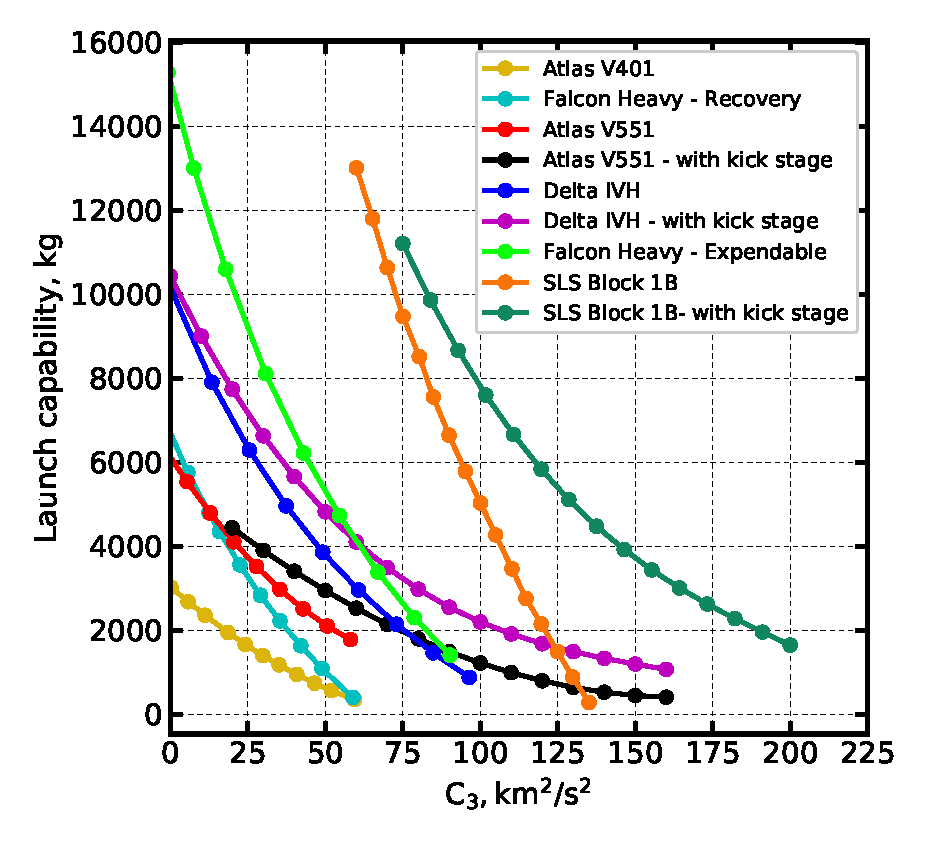
\includegraphics[width=5in]{images/C3-Curves.eps}
\caption{Sample image.}
\label{sample-image}
\end{figure}

\section{Verification and Validation}
\begin{table}[htpb!]
\caption{Sample table title} \label{sample-table}
\begin{center}
\begin{tabular}{|c|c|c|c|c|c|}
  \hline
% after \\: \hline or \cline{col1-col2} \cline{col3-col4} ...
   & $k_{g}$ & $k_{o}$ & $c_{3}$ & $c_{4}$ & $c_{5}$ \\
  \hline\hline
  Careful/Sparse & 0.334 & 0.597 & 1.101 & 9.621 & 8.170 \\ \hline
  Careful/Dense & 3.124 & 3.195 & 1.094 & 5.899 & 7.318 \\ \hline
  Aggressive/Sparse & 0.840 & 9.153 & 2.853 & 8.274 & 0.187 \\ \hline
  Aggressive/Dense & 4.838 & 2.841 & 0.670 & 7.952 & 0.386 \\ \hline
  Hand-Tuned & 0.767 & 0.060 & 0.340 & 2.000 & 0.250 \\
  \hline
\end{tabular}
\end{center}
\end{table}

\section{Sample Test Results with Prototype Tire}

\section{Conclusions}

This is the conclusion.

\subsubsection*{Acknowledgments}
This is the acknowledgement.

\bibliographystyle{apalike}
\bibliography{references}

\end{document}